\section{Scaling to Large KGs}\label{sec:system}
We discuss systems considerations when using KG reasoning embedding models over large-scale KGs. Beyond scalable training, we also require that inference over Query2Box models is scalable and incremental. This requirement is important to enable practical deployments over dynamic billion-scale KGs. We next discuss the main components of the architecture we adopt (see Figure~\ref{fig:sys_overview}).

 \begin{figure}
        \centering
      \includegraphics[width=0.7\columnwidth]{submissions/Ali2023/figures/embedding_models_q2box_v2.pdf}
      \caption{An overview of using Knowledge Graph Embedding models for large-scale fact ranking.}
    \label{fig:sys_overview}
\end{figure}

The multi-hop nature of embedding models such as Query2Box poses unique challenges when training these models over billion-scale KGs. In the case of shallow KG embedding models, graph partitioning is a common method for scaling training~\cite{zhu2019graphvite, lerer2019pytorch}. Unfortunately, these methods are not applicable in the case of reasoning-based embeddings. When using Query2Box it is important that we can generate training samples by performing multi-hop traversals of the graph. Such traversals can span multiple partitions. At the same time, it is not always practical to pre-compute such samples in advance. To alleviate this issue, we opt for a single-machine multi-GPU deployment during training and leverage the recently introduced SMORE engine~\cite{ren2021smore} to perform training. SMORE provides a mixed GPU-CPU solution that leverages both the main memory and GPU memory to scale training. In addition, training examples are generated on the fly thus avoiding unnecessary pre-compution. Indicative throughput measurements and scaling of SMORE is shown in Figure \ref{fig:speedup}. A requirement here is that the machine have sufficient main and on-device memory to store the entire graph and thus avoid partitioning. While this requirement is satisfied by modern hardware configurations it is a cost-hungry option. We believe disk-based or distributed training of reasoning-based KG embeddings is an exciting research direction. Once training is complete, the embedding models are archived and then used for inference.

\begin{figure}[t]
\centering
    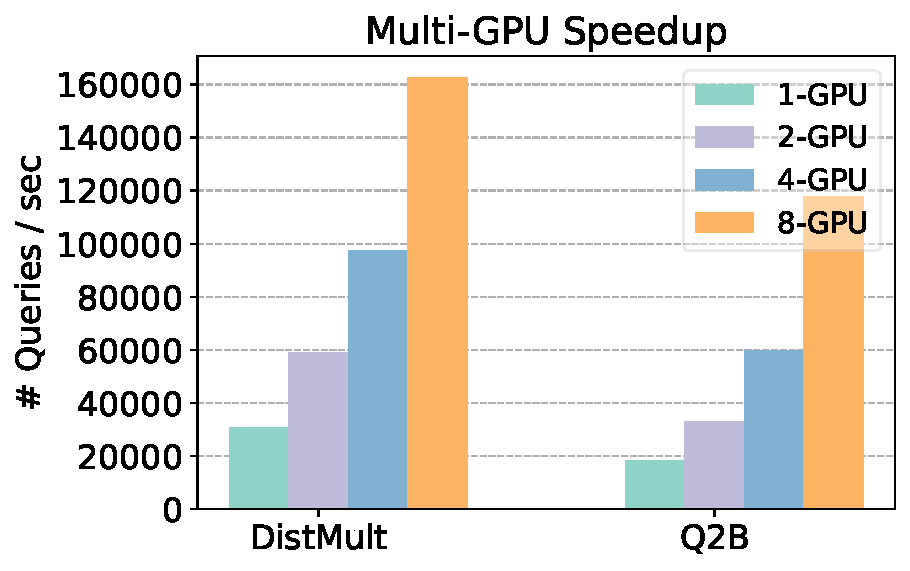
\includegraphics[width=0.3\columnwidth]{submissions/Ali2023/figures/wiki-speedup.pdf}
    \caption{Multi-GPU scaling of SMORE for training the DistMult and Query2box embedding models.
    }
\label{fig:speedup}
\end{figure}

At inference time, we opt for a batch inference setting. We first compute a series of candidate queries that correspond to the set of facts that we want to enable ranking over. We leverage a computation graph engine to materialize all \emph{candidate} queries (\ie, \texttt{(subject, predicate, object} triples) and use the learned Query2Box model to obtain a score for each query. The number of candidate facts can exceed the size of the original KG as we consider multiple subject, object configurations that may not appear in the original graph. To deal with the volume of generated queries we opt for a scatter gather-based multi-GPU inference across multiple machines in a GPU cluster. The trained model is loaded in the executor allocated to each machine and the candidate facts are partitioned across machines. The corresponding inference results are gathered into a single relational store and then used for downstream processing. Given the stability of the Query2Box representations (see Section~\ref{sec:experiment}), we maintain the fact ranking results via periodic retraining of the Query2Box models followed by batch inference. Inference results for fact ranking are versioned across different training and batch inference runs.

\iffalse

\revise{
Performing batch inference for related entity search (Section \ref{sec:related_entities}) has additional requirements due to the unique characteristics of the related entity search task: (i) hybrid queries and their relational predicates require inference techniques beyond traditional vector similarity search-based solutions, and (ii) the volume and variety of candidate queries that are generated from available prior workloads render static, ``one size fits all'' solutions ineffective. 
To this end, we employ \hybridindex~\cite{mohoney2023high} hybrid vector similarity search system for  batch inference over KG embeddings, which provides the following suite of optimizations for \textit{high-throughput batch processing of hybrid queries}:
}

% The batch processing requirement of our workload is in fundamentally different from the existing industrial-scale systems focus on latency optimized online hybrid query processing. Therefore, in contrast to the other fact ranking tasks, our primary challenge here is performing \textit{high-throughput batch processing of hybrid queries} on KG embedding trained for the use-case. The requirements of related entity search use-case necessitate new optimizations that current vector database systems do not cover. To this end, we proposes the following suite of solutions including a \emph{workload-aware vector index} and a \emph{multi-query optimization technique}:

\textbf{Workload-aware vector index:}
First, we introduce a new workload-aware index for vector databases.
Specialized vector indexes that either partition the data or form multi-level indexes over centroids are commonly used in vector databases to speed-up vector similarity search \cite{guo2022manu, wang2021milvus, yang2020pase}. Here, we use past workload information to guide the partitioning of the vectors in the underlying index in a  way that hybrid queries can be answered by accessing as few partitions as possible. We extend the concept of \emph{query-data routing trees (qd-trees)}~\cite{qd-tree} to consider both vectors and relational predicates from a hybrid query workload when generating physical data layout at data loading time. The resulting data layout partitions the vectors using the distribution of the attributes associated with vectors, the attribute constraints, and similarity of vectors present in the hybrid query workload. We then use the resulting partitioning scheme to generate an index layout that enables us to process a batch workload of hybrid queries by accessing vectors from as few partitions as possible.

\textbf{Batch query optimization:}
Second, we introduce a multi-query optimization technique that (i) batches queries with similar attribute and vector similarity constraints; and (ii) performs batch vector distance computation against a posting list of vectors obtained from a clustering-based index over the vectors. 
This optimization is motivated by the fact that the set of candidate queries are computed from past user queries and evaluated in a batch setting, which enables computation sharing across queries.
% This optimization is motivated by the fact that our target hybrid query workloads need to be evaluated in a batch setting, enabling computation sharing across queries. 
Note that this optimization is orthogonal to the workload-aware vector index and is applicable to any clustering-based vector index.

\fi